
\subsubsection{5.1 Main Results}

Table 1 presents aggregate statistics for heavy-tailed exponent measurements across 53 ViT models.

\begin{table}[htbp]
\centering
\resizebox{\columnwidth}{!}{%
\begin{tabular}{ll}
\toprule
Metric & Value \\
\midrule
Models processed & 53 \\
Mean $\alpha$ & 4.327 \\
Median $\alpha$ & 3.521 \\
$\sigma (\alpha )$ global & 2.868 \\
$\alpha$ range & [2.20, 18.92] \\
\bottomrule
\end{tabular}
}
\end{table}

\textbf{Gate verdict: FAIL.} The global variance $\sigma$ = 2.868 exceeds the threshold of 0.5 by a factor of 5.7.

\subsubsection{5.2 Within-Family Variance}

When stratifying by model family (organizational training origin), variance decreased substantially for the google/vit-* family.

\begin{table}[htbp]
\centering
\resizebox{\columnwidth}{!}{%
\begin{tabular}{llll}
\toprule
Family & n & Mean $\alpha$ & $\sigma (\alpha )$ \\
\midrule
google/vit-* & 6 & 3.700 & 0.24 \\
Global (all models) & 53 & 4.327 & 2.868 \\
\bottomrule
\end{tabular}
}
\end{table}

This represents approximately 12-fold variance reduction (2.868 / 0.24 $\approx$ 11.95) through family stratification. However, only one family had sufficient samples for reliable within-family variance estimation.

\subsubsection{5.3 Outlier Analysis}

Several models exhibited extreme $\alpha$ values (>10):

\begin{table}[htbp]
\centering
\resizebox{\columnwidth}{!}{%
\begin{tabular}{lll}
\toprule
Model & $\alpha$ & Training Task \\
\midrule
jaranohaal/vit-base-violence-detection & 12.64 & Violence detection \\
mlx-vision/vit\_base\_patch16\_224-mlxim & 14.84 & MLX conversion \\
\bottomrule
\end{tabular}
}
\end{table}

These outliers correspond to task-specific fine-tuning or format conversion, not architectural variants of standard ViT.

\subsubsection{5.4 Summary of Findings}

\begin{table}[htbp]
\centering
\resizebox{\columnwidth}{!}{%
\begin{tabular}{lll}
\toprule
Research Question & Answer & Evidence \\
\midrule
RQ1: Can $\alpha$ be computed for ViT? & Yes & 53/150 models processed successfully \\
RQ2: Is variance bounded ($\sigma$ < 0.5)? & No globally, Yes within family & $\sigma$ = 2.868 global, $\sigma$ = 0.24 for google/vit-* \\
RQ3: Does family control help? & Yes & ~$12\times$ variance reduction \\
\bottomrule
\end{tabular}
}
\end{table}

\begin{figure}[htbp]
\centering
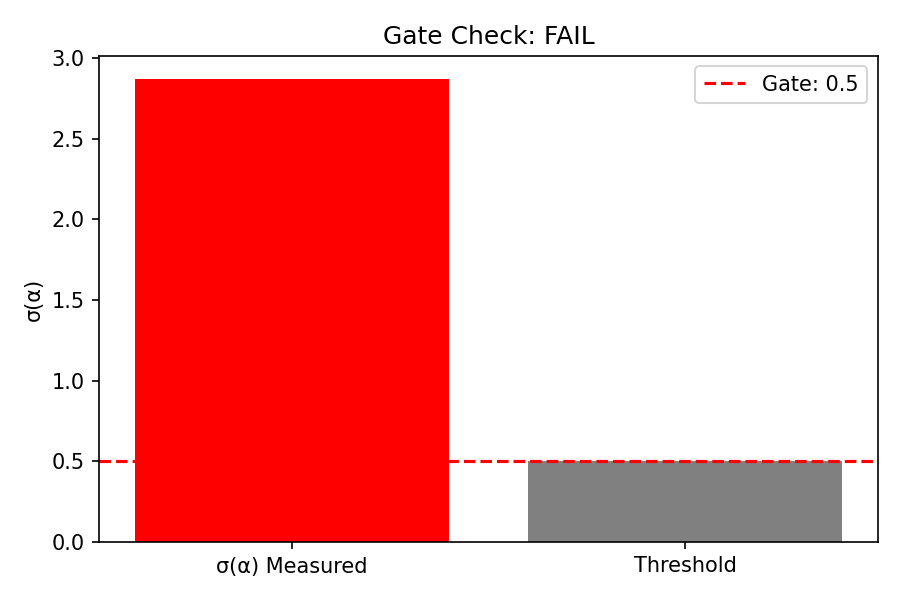
\includegraphics[width=\columnwidth]{figures/gate_check.png}
\caption{Gate Check Visualization}
\label{fig:gate_check}
\end{figure}

\begin{figure}[htbp]
\centering
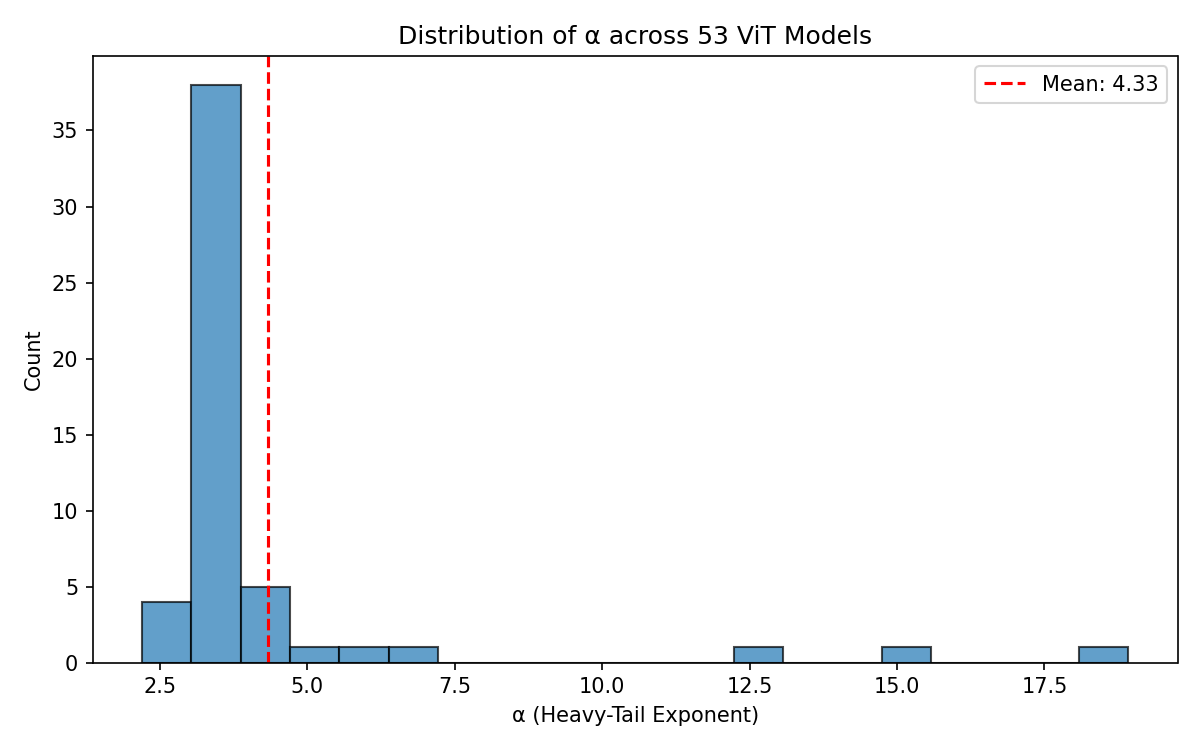
\includegraphics[width=\columnwidth]{figures/alpha_histogram.png}
\caption{Alpha Distribution}
\label{fig:alpha_histogram}
\end{figure}

